\section{The \codegen Methodology }
\label{sec:appII-approach}

This section presents \codegen, a set of causal inference tools to \textit{interpret the prediction performance} of \nlms by connecting causal models to data. \codegen instantiates the concepts and theory discussed in the previous section by introducing three stages (St$_1$-St$_3$): (i) \textit{Modeling Causal Variables}, (ii) \textit{Computing Causal Inference}, and (iii) \textit{Evaluating Causal Effects}. Because \codegen focuses its analysis upon the probability distribution of Next Token Predictions (NTPs) and Cross-Entropy, it falls into the category of model-specific (\ie to \nlms) post-hoc interpretability methods \citep{molnar2019interpret}. We have implemented \codegen in an open source library, which we will make freely available upon acceptance of this paper~\citep{icodegen}.

\subsection{Stage 1 (St$_1$): Modeling Causal Variables}
In this stage, assumptions about relationships among data are defined in a structural causal model similar to Fig.~\ref{fig:scm}, which is later processed in St$_2$ to compute $p(Y|do(T))$. Causal assumptions must be made explicit, which means defining the treatments $T$ (\ie binary: buggy/non-buggy, discrete: layer modifications), potential outcomes $Y$ (\ie global (Cross-Entropy) and local (NTPs) performance), and the common causes $Z$ that can affect the treatments and potential outcomes. For all our SCMs in this study, we assumed that common causes are SE quality metrics since they have the potential to influence models global and local performance, \ie a \nlm may be influenced by more or less for loops, as well as influence treatments, \ie more code has been shown to be correlated with more bugs. In summary, St$_1$ consists of setting down assumptions about the causal relationships of software data employed to interpret \nlms. SCMs help us to describe the relevant features of the software data and how they interact among each other. In the following subsection, we formally define our treatments and potential outcomes.  

\textbf{a. Defining SE Counterfactual Interventions or Treatments.}
\nlms are notorious for not working well outside the distribution they were trained and tested on. For example, if a model trained on a well-commented dataset is applied to predict segments of poorly commented code, this mismatch could potentially impact performance. As such, we assert that observing model performance across datasets with different characteristics can aid in understandability. Hence, we defined \textit{SE Counterfactual Interventions} $T$ to better understand model performance across different settings. We formulate these interventions as testbeds (\ie datasets) organized in sample pairs \textbf{treatment} $T=0$ (\ie BuggyCode) and \textbf{control} $T=1$ (\ie FixedCode). Note that we define testbeds according to different applications often described in SE research. The testbed preparation process is highly dependent on code properties. The general process comprises of identification of some specific \textit{intervention} (\ie program repair) and 2) construction or collection of the necessary data via mining repositories or other means that contain these interventions. More complex interventions will likely be more challenging to prepare. In \codegen, \textit{counterfactual interventions} produce explanations motivated by both semantic perturbations (or treatments) $T_{[data]}$ to our SE Application Settings (\eg Buggy/Fixed, Commented/Uncommented, Clone1/Clone2) and model hyper-parameter variations $T_{[hyp]}$ on \nlms  (\eg layers, units, or heads).

\textbf{b. Defining Potential Outcomes / Model Performance} Cross-Entropy ({Fig.~\ref{fig:performance}-\circled{3}}) and Next Token Prediction ({Fig.~\ref{fig:performance}-\circled{2}}) are relevant values produced at inference time that reflect the effectiveness of a model. By relating these values to counterfactual interventions $T$ (\ie program repair), we can gain an understanding of how well a studied model is \textit{generating code} under these treatments. We refer to Cross-Entropy loss as a measure of a model's \textit{Global Performance} $Y_g: w \to - \sum_{t \in |w|} P(w_t | d_t) \log Q(w_t | w_{<t})$ as these losses capture the overall performance of a \nlm over an entire sequence of tokens $w$. Due to the discrete nature of the data, the expression $P(w_t | w_{t-1:1} )$ can be estimated using a classifier. The classifier, in our particular case, is a \nlm \citep{Bengio2003AModel}. Hence, rather than using \textit{n}-grams or Markov Models to approximate $P(w_t | w_{t-1:1})$ \citep{Karampatsis2020Open-VocabularyAbstract}, it is convenient to use a latent model $P(w_t | w_{t-1:1} ) \approx P(w_t | d_t )$, where $d_t$ is known as a \textit{hidden state} that embeds the sequence information from past observations up to the time step $t$. Depending on \textit{how} the sequence is processed, the hidden state $d_t$ can be computed using either an autoregressive network (\ie such as a Transformer ($TF$)~\citep{vaswani2017transformers}) or a Recurrent Neural Network ($RNN$). Conversely, Next Token Prediction (NTP) values signal \textit{Local Performance} $Y_l:w_{<t} \to P(w_t | w_{t-1:1})$ within token-level contexts. NTPs capture local predictions for individual tokens that are affected by complex interactions in \nlms and are equivalent to the estimated predicted value (or softmax probability) $\sigma(k)_t$ for each token. Bear in mind that the size of the vector $\sigma(k)_t$ is the vocabulary $|\mathcal{V}|$, in which $k$ represents the non-normalized log probabilities for each output token $t$. NTPs capture the value of the expected token $w_t$ instead of the maximum value estimated in the vector $\sigma(k)_t$.

\begin{figure}[h]
		\centering
		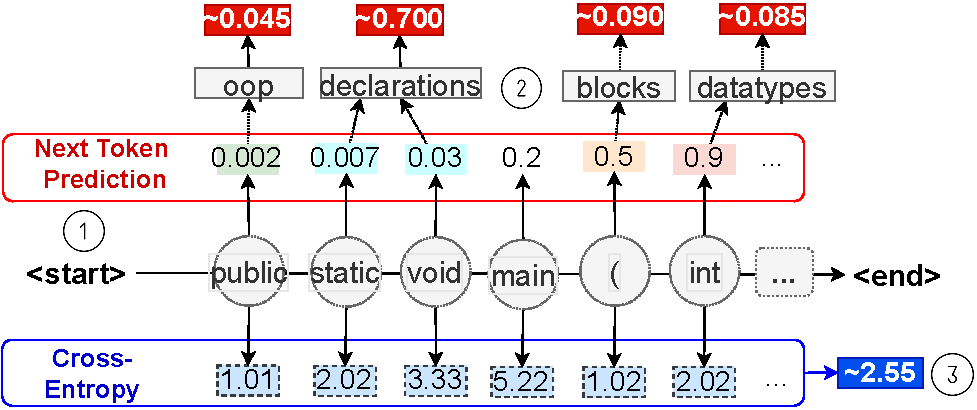
\includegraphics[width=0.9\textwidth]{graphics/preliminaries/fig_2_performance.pdf}
		\vspace{-0.3cm}
		\caption{Potential Outcomes are Prediction Performance of  \nlms: Cross-Entropy $(Y_g)$ and Next Token Predictions $(Y_l)$.}
        \vspace{-0.1cm}
        \label{fig:performance}
\end{figure}

A major conjecture in interpretability research is that \nlms are more understandable when they \textit{reflect human knowledge} \citep{Kim2018InterpretabilityTCAV}. One way of determining whether a model reflects human knowledge is testing it to see whether or not it operates (or predicts) \textit{similar to how a human would operate}. \codegen accomplishes this by mapping the complex interactions present in both Global $Y_g$ and Local $Y_l$ Potential Outcomes of a \nlm to human interpretable PL features and testbeds. Below we provide a motivating example for this mapping function, which we formally introduce in Definition \ref{def:taxonomy}:

\begin{exmp}
\label{exmp:outcome}
Consider the situation where a developer inserts a \texttt{\small `('} character after the \texttt{\small `main'} keyword in a function declaration in Java ({\circled{1}}-Fig.~\ref{fig:performance}). Inherently, a developer mentally rationalizes several things such as the concept of a function declaration and expected Java syntax. If a \nlm is able to make a similar prediction, it suggests to us that it has \textit{statistically learned} some understanding of the concept of a function declaration and corresponding syntax. Thus, we assert that by ascribing human-interpretable properties, and in particular code-related properties, to model predictions, and then analyzing the statistical properties of those predictions, we can begin to learn how well a given \nlm reflects human knowledge. We propose a \textit{Structural Code Taxonomy} $\mathcal{H}$ to bridge this interpretability gap.
\end{exmp}

\marginnote{
    \begin{definition}
    \label{def:taxonomy}
    \textbf{Structural Code Taxonomy.} In programming languages (PL), different types of tokens retain different semantic meanings. For instance \texttt{\small `='} and \texttt{\small `<'} are common \operators. As such, we can group tokens into semantically meaningful \textit{categories}. Fig.~\ref{fig:taxonomy} depicts an initial version of \codegen's taxonomy derived from Java. These features will allow \codegen to assign semantic meaning to predicted tokens $\hat{w_t}$. The taxonomy comprises high-level properties of code using a \textbf{mapping function} $\phi_{\mathcal{H}}: \vec{w} \to \vec{h} $, where the vector $\vec{w}$ corresponds to tokens of the vocabulary $\mathcal{V}$. Each token in a sequence $w$ is assigned to a taxonomy category $h \in \mathcal{H}$.
    \end{definition}
}

With our categories $\mathcal{H}$, researchers and practitioners can easily associate \nlm performance (\ie $Y_g$ or $Y_l$) to particular structural code attributes. As such, by using our structural code taxonomy, \codegen allows for \nlm predictions to be interpreted in a developer-centric way. These categories represent a “base” case as the keywords of any PL can likely be grouped into interpretable categories. This is why anyone using \codegen can \textit{easily define their own mapping function} $\phi_{\mathcal{H}}$ (\eg using coupling and cohesion metrics), and stipulate them in a JSON-like configuration file. For instance, a researcher working to analyze how well \nlms learn to predict cryptographic APIs could define a taxonomy based upon “safe” and “unsafe” APIs.

 \begin{marginfigure}
		\centering
		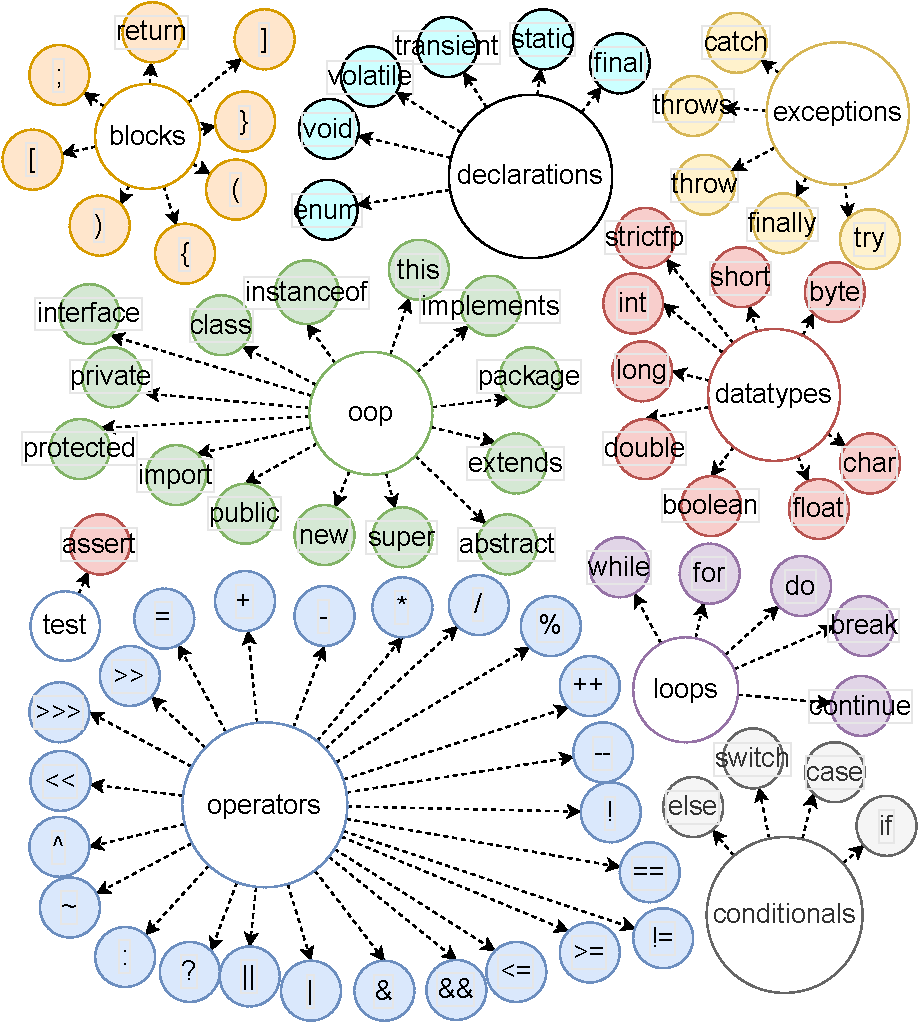
\includegraphics[width=\textwidth]{graphics/preliminaries/fig_3_taxonomy.pdf}
		\caption{Structural Code Taxonomy $\mathcal{H}$ for Java}
        %\vspace{-0.5cm}
        \label{fig:taxonomy}
\end{marginfigure}

\subsection{Stage 2 (St$_2$): Computing Causal Inference (CI)}
%Definition of Causal Inference
According to Pearl \& Mackenzie \citep{Pearl2018Causality}, CI seeks answers to questions of association (\textit{what is?}), counterfactual interventions (\textit{what if?}), and pure counterfactuals (\textit{why?}). The authors introduce the concept of \textit{levels of causation} to match distinct levels of cognitive ability with concrete actions: seeing~(\textit{level 1}), doing~(\textit{level 2}), and imagining~(\textit{level 3}). Our proposed analysis is primarily concerned with levels 1 \& 2. Level 1 causation, namely association, $p(Y|T)$ is estimated by using typical correlation methods (\eg Pearson, Spearman, or Covariance) in addition to functional associations such as $y=g(t)$, which can be predicted with regressions or ML methods. For binary treatments similar to the ones we used in $T_{[data]}$ (\eg Buggy/Fixed, Commented/Uncommented, Clone1/Clone2), we opt to employ Pearson correlations and Jensen-Shannon distance as association estimand for level 1 causation. We will now formally define each of these below \david{Contextualize the functions below}.

\marginnote{
\begin{definition}
\label{def:js}
\textbf{Jensen-Shannon Distance (JS).} The Jensen-Shannon divergence (JSD) overcomes the asymmetric computation of the KL divergence and provides a measure of difference between distributions Eq.~\ref{eq:js_divergence}. The JS distance is the square of the JS divergence $p(Y|T)\approx JS(Y^{T=0},Y^{T=1}) = JSD(Y^{0},Y^{1})^2$. JS is proportional to the influence of $T$ on $Y$, which measure the separation of the distributions $Y^{0},Y^{1}$. The notation $Y^{T=0}$ refers to the potential outcomes observed under the treatment $T=0$. 

\end{definition}
}

\begin{subequations}
    {%\tiny %footnotesize
    \begin{align}
     JSD(Y^{0}=y^0,Y^{1}=y^1) &&= \label{eq:js_divergence-1}\\
     \frac{1}{2}\left[ D_{KL}\left(y^0||\frac{y^0+y^1}{2}\right) + D_{KL}\left(y^1||\frac{y^0+y^1}{2}\right)\right] &&= \label{eq:js_divergence-2}
    \end{align}
    }
\label{eq:js_divergence}
\end{subequations} 

\begin{exmp}
\label{exmp:js}Imagine we wish to understand the correlation between syntactic changes, \ie variable renaming, alterations in white space, \etc and a \nlms performance. One way we can study this is through computing the association of Cross-Entropy values $Y$ under two treatments, the first $T=0$, would be an unaltered code snippet and the second $T=1$ would be its Type III clone. Computing this association can be done using the JS distance $p(Y|T)\approx JS(Y^0,Y^1)$ as defined in Def.~\ref{def:js} for four models. Fig.~\ref{fig:jssimilarity} shows the distributions of $Y^0$ and $Y^1$ with their distances after applying bootstrapping as an example.

\begin{figure}[h]
  \centering
  \begin{subfigure}[b]{0.46\linewidth}
    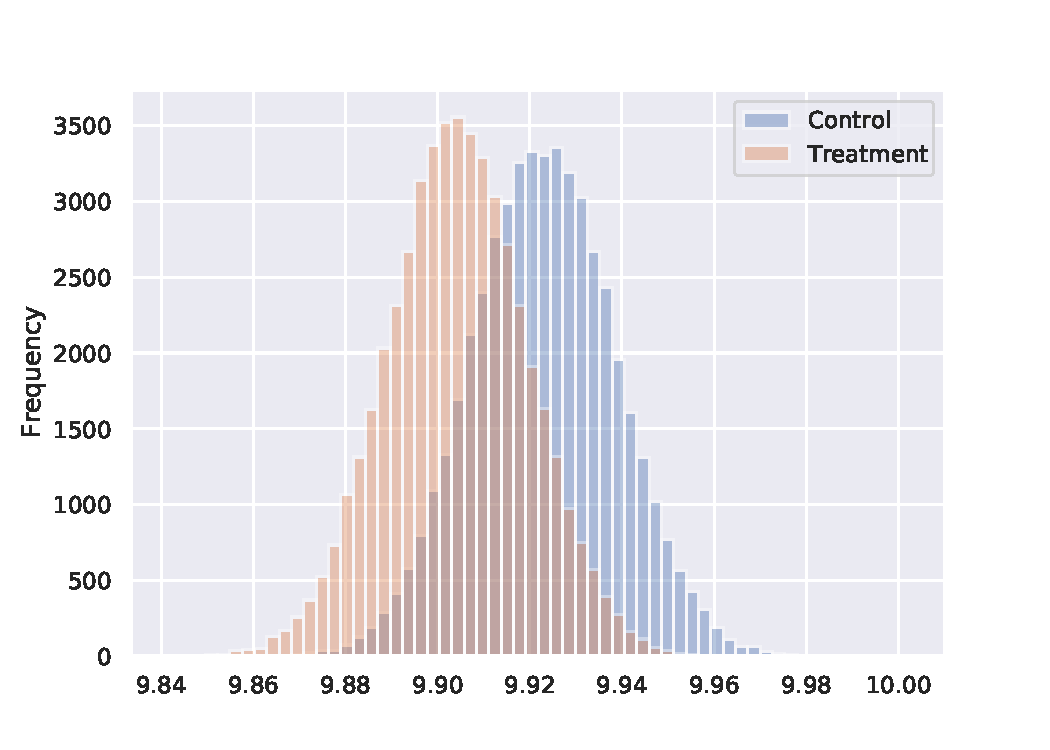
\includegraphics[width=\linewidth]{graphics/preliminaries/association/cross-entropy-rnn1-distribution-clone3-300dpi.pdf}
    %  \caption{RNN1.}
  \end{subfigure}
  \begin{subfigure}[b]{0.46\linewidth}
    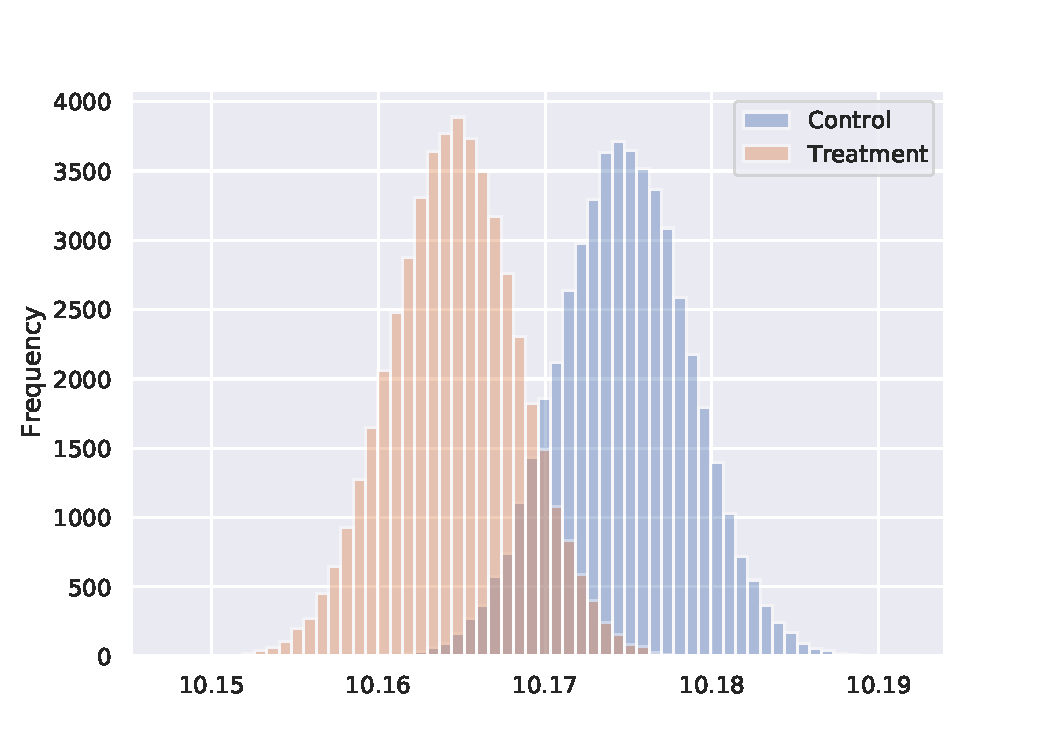
\includegraphics[width=\linewidth]{graphics/preliminaries/association/cross-entropy-gru1-distribution-clone3-300dpi.pdf}
    % \caption{GRU1.}
    % \vspace{0.2cm}
  \end{subfigure}
  \begin{subfigure}[b]{0.46\linewidth}
    % \vspace{-0.2cm}
    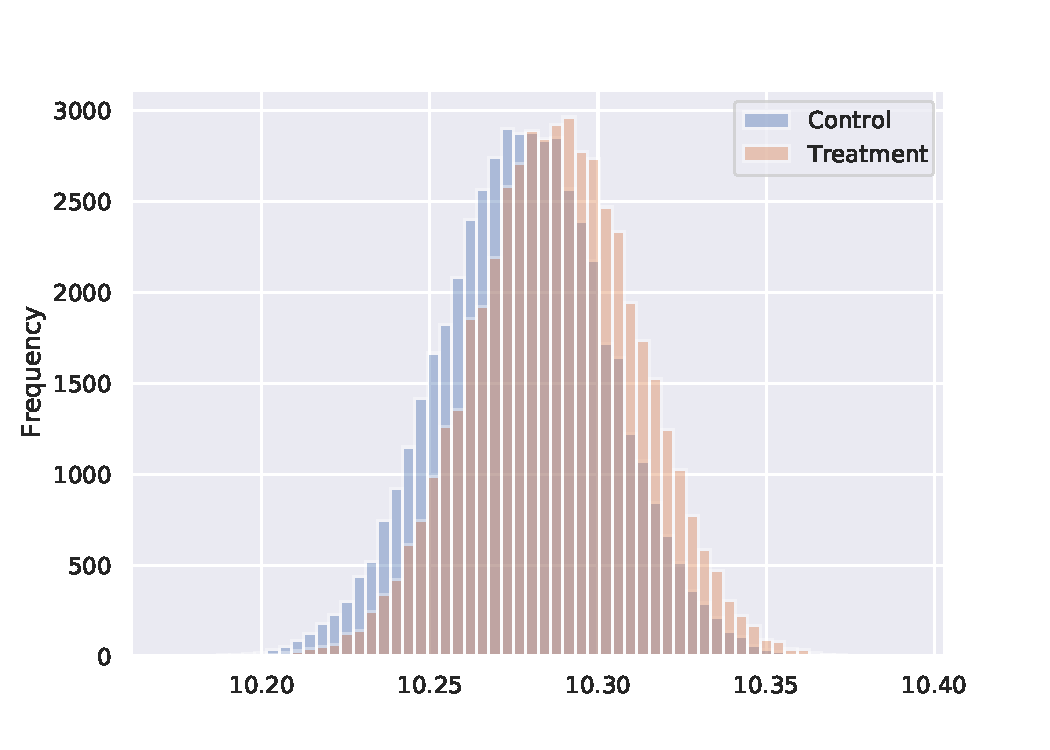
\includegraphics[width=\linewidth]{graphics/preliminaries/association/cross-entropy-tf1-distribution-clone3-300dpi.pdf}
    % \caption{TF1.}
  \end{subfigure}
  \begin{subfigure}[b]{0.46\linewidth}
    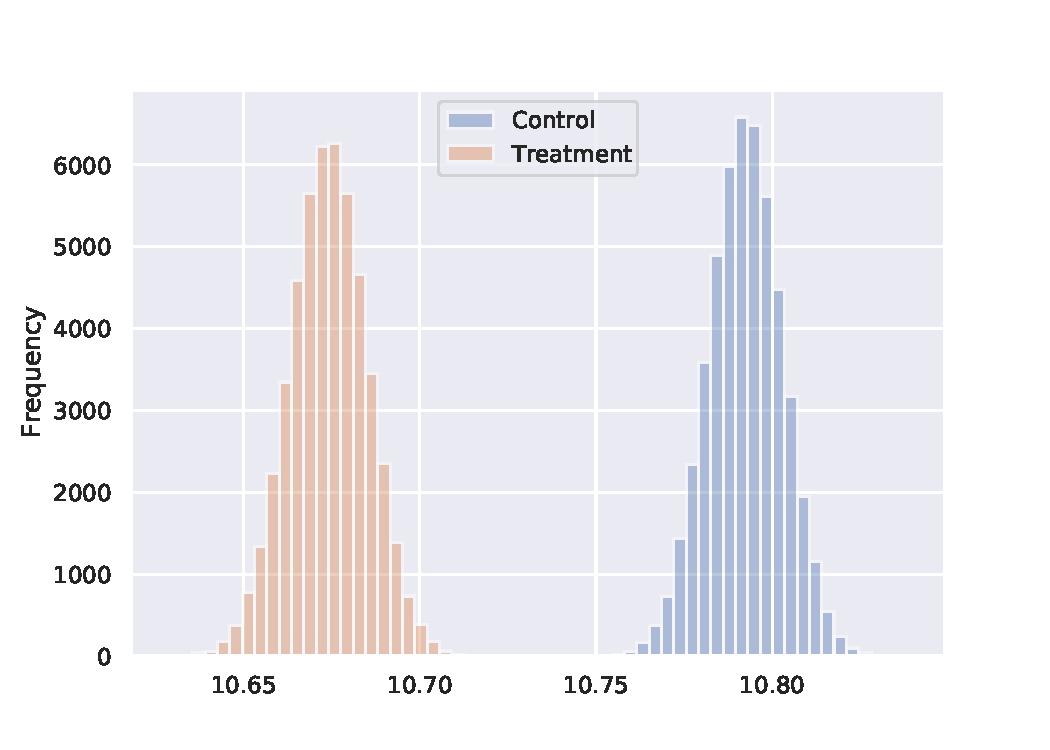
\includegraphics[width=\linewidth]{graphics/preliminaries/association/cross-entropy-tf2-distribution-clone3-300dpi.pdf}
    % \caption{TF2.}
  \end{subfigure}
  \vspace{-0.2cm}
  \caption{\datainterII Intervention (\BigCloneIIITB) for Global Performance: Bootstrapped Cross-Entropy. Top Left: \rnn ($JS=0.3$), Top Right: \gru ($JS=0.8$), Bot Left: \tf ($JS=0.6$), Bot Right: \tfi ($JS=1$).}
  \label{fig:jssimilarity}
  \vspace{-0.3cm}
\end{figure}

\end{exmp}

Now, if we want to go beyond \textit{``what is''} type questions, we must move past simple correlations and association. This requires the $do-operator$ found in level 2, causation $p(y|do(t))$. Specifically, it is estimated for a population (\ie SE dataset) by computing an \textit{Average Treatment Effect} based on the Def.~\ref{def:effect} introduced in Sec.~\ref{sec:pre-ci4se}.

\marginnote{
\begin{definition}
\label{def:ate}
\textbf{Average Treatment Effect (ATE)} Defining the first intervention as $do(T=1)$ and the second by $do(T=0)$, the Average Treatment Effect is the population average of the difference of causal effects of each code snippet $x$.  
\end{definition}
}

\david{Contextualize the functions below}
\begin{subequations}
    \begin{align}
     ATE = \mathbb{E}_{x\sim p(x)}[Y=y|x,do(T=t)]  &= \label{eq:ate-1}\\
     \mathbb{E}_{x\sim p(x)}[ \mathbb{E}[Y|x,do(T=1)] - \mathbb{E}[Y|x,do(T=0)] ] &= \label{eq:ate-2}\\
     \mathbb{E}_{x\sim p(x)}[ \mathbb{E}[Y^{1}|x,T=1] - \mathbb{E}[Y^{0}|x,T=0] ] &= \label{eq:ate-3}
    \end{align}
\label{eq:ate}
\end{subequations} 


ATE can be computed in two steps as follows:

\textbf{a. Identifying Causal Effects.} Once the SCM (similar to Fig.~\ref{fig:scm}) is constructed, \codegen applies various techniques (\ie backdoor-criterion and instrumental variables) to determine the adjustment formula Eq.~\ref{eq:effect}, which will control for confounding common causes when computed. For our case study, the causal effect $p(Y|do(T))$ is computed, which will be done in the next step, based on the following causal graph: data-based $T_{[data]}$ and parameter-based $T_{[hyp]}$ treatments; SE covariates $Z \in SE_{metrics}$; and potential outcomes $Y_l, Y_g$.

\textbf{b. Estimating Causal Effects.} Next, \codegen estimates the causal effect using statistical and ML methods based on the adjustment formula from the previous step. \codegen computes \textit{Propensity Score Matching} for binary SE treatments (\ie Buggy/Fixed) and \textit{Linear Regressions} for SE discrete treatments (\eg layers, units, or heads). We refer interested readers to the \textit{doWhy} documentation for the full process details \citep{dowhy}. For completeness, we will now show how to estimate a causal effect assuming a binary treatment as an example. Eq.~\ref{eq:ate} shows the formal definition of an \textit{ATE}. We can derive the final expression by applying the law of total expectations and the ignorability assumption  $Y \perp\!\!\!\perp  Z|T$, where the potential outcomes $Y$ are independent of treatment assignments conditioned on covariates $Z$ \citep{Pearl2009Causality}. That is, the effects of the hidden common causes $Z$ and missing data are ignored. In Eq.~\ref{eq:ate}, the term $\mathbb{E}[Y^1|x,T=1]$ represents the expected value of a potential outcome under an observable treatment (\ie FixedCode). Similarly, the term $\mathbb{E}[Y^0|x,T=0]$ represents an expected value of a potential outcome under an observable control (\ie BuggyCode). Both terms are quantities that can be \textit{estimated from data}. Covariate adjustment (in Eq.~\ref{eqn:do-all-lines}), propensity score (in Eq.~\ref{eq:effect-3}), and linear regression are some of the estimation methods that we employ to estimate the $ATE$. Their usage depends upon the type of the treatment variable (\ie binary, discrete, or continuous) and causal graph assumptions.

\subsection{Stage 3 (St$_3$): Evaluating Causal Effects}
The previous causal estimation can be validated using \textit{refutation methods} that calculate the robustness of the causal estimate. In essence, the refutation methods apply random perturbations to the original causal graph to test for robustness of the estimated $ATE$. We chose four methods for our analysis: Adding a random common cause or covariate $\mathcal{R}_1$, adding an \textit{unobserved} common cause or covariate $\mathcal{R}_2$, replacing the treatment with a random variable or placebo $\mathcal{R}_3$, and removing a random subset of the data $\mathcal{R}_4$. For robustness, we expected that $\mathcal{R}_1$, $\mathcal{R}_2$, and $\mathcal{R}_4$ values were close to the $ATE$ (Eq.~\ref{eq:ate}). Conversely, the placebo $\mathcal{R}_3$ should tend to zero.

In addition to measuring refutation methods, it is relevant to identify cases of \textit{spurious correlations} (\ie \textit{Confounding Bias}) or cases where $p(Y|T)\neq p(Y|do(T))$. Typically, association is not causation due to the influence of a common cause or confounding variable $Z$. Such a variable is the one that is being controlled for or adjusted by means of Eq.~\ref{eqn:do-all-lines}. Nonetheless, we can still compute the correlation $d(Y|Z)$ to assess the variables that are actually affecting potential outcomes. 

 \begin{marginfigure}
		\centering
		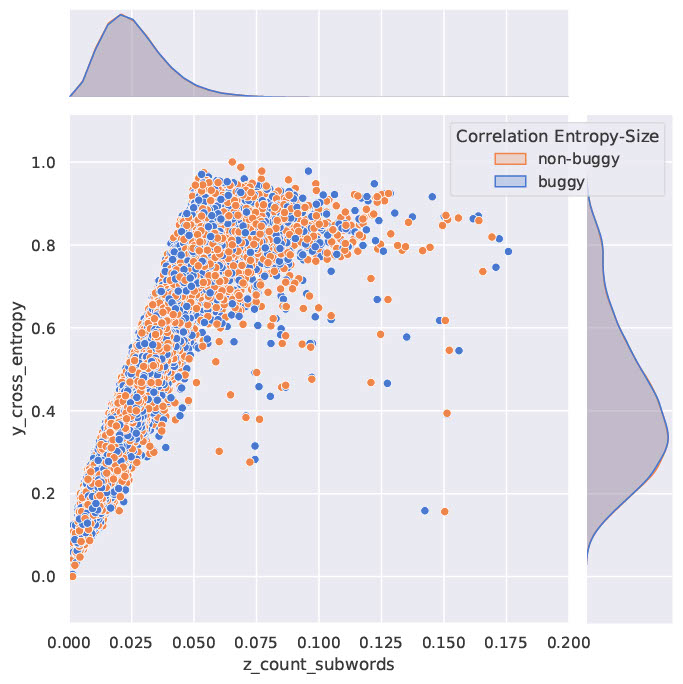
\includegraphics[width=\textwidth]{graphics/fig_4_covariates_corr.jpg}
		\caption{ \textit{Spurious Correlation} between the \textit{Number of Subwords} common cause and Cross-Entropy values ($p(Y|Z)\approx0.87$) for the \datainterI intervention generated from \tf. } 
        \vspace{-0.5cm}
        \label{fig:covariate}
\end{marginfigure}

\begin{exmp}
\label{exmp:confounding}

Consider the \datainterI intervention where $T$ is Buggy/Fixed code, $Y$ is the cross-entropy of each of method of the dataset \BuggyTB, and $Z$ is the \textit{Number of Subwords} for each method. There exists a spurious correlation after calculating JS and ATE, $p(Y|T)\approx0.67$ and $p(Y|do(T))\approx-0.0002$. One possible explanation is that the common cause $Z$ is confounding the relationship between the treatment and the outcome. Fig.~\ref{fig:covariate} depicts the influence of $Z$ on the potential outcome $Y$ for BuggyCode ($p(Y|Z,T=Buggy)\approx0.87$) and FixedCode ($p(Y|Z,T=Fixed)\approx0.86$). Blue and orange points in the plot are code snippets from the dataset. These points are equally distributed, which suggest that the \datainterI intervention has a negligible impact on the Cross Entropy. 
\end{exmp}